% ============================================================
%  1-bit register - logic diagram.
%  A 2:1 multiplexer (select = LD) chooses what the D flip-flop sees
%  on the next clock edge:
%      LD = 1  -> pass the new data D   (load)
%      LD = 0  -> pass Q back to itself (hold)
%  So the bit only changes when LD = 1, even though CLK keeps ticking.
%  Built from: the D flip-flop board + a 2:1 MUX (2 AND + 1 OR + 1 NOT).
%  Compile:  pdflatex circuit.tex
% ============================================================
\documentclass[border=30pt]{standalone}
\usepackage{circuitikz}
\usepackage{amsmath}
\usetikzlibrary{calc}

\begin{document}
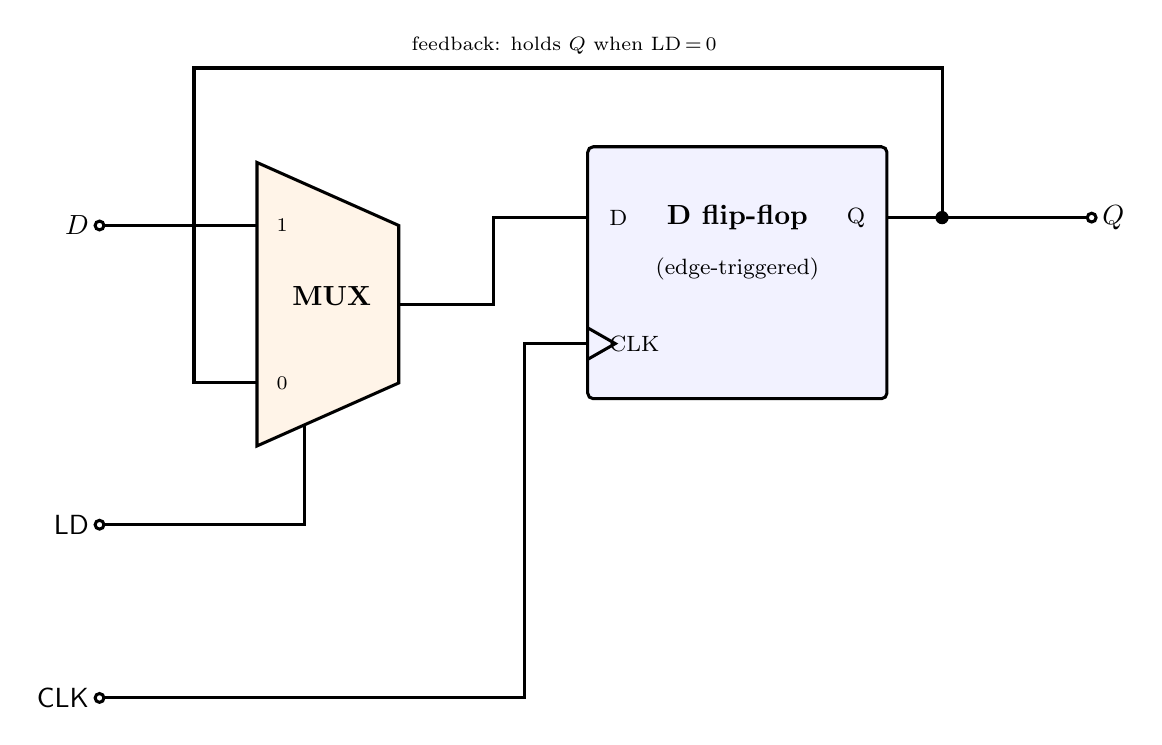
\begin{tikzpicture}[line width=1.1pt, font=\sffamily]

  % ---------- 2:1 MUX (load select) ----------
  \draw[fill=orange!9] (3.0,1.8) -- (3.0,5.4) -- (4.8,4.6) -- (4.8,2.6) -- cycle;
  \node[font=\bfseries] at (3.95,3.7) {MUX};
  \node[font=\scriptsize] at (3.32,4.6) {1};
  \node[font=\scriptsize] at (3.32,2.6) {0};

  % ---------- D flip-flop block ----------
  \draw[rounded corners=2pt, fill=blue!5] (7.2,2.4) rectangle (11.0,5.6);
  \node[font=\bfseries] at (9.1,4.7) {D flip-flop};
  \node[font=\footnotesize] at (9.1,4.05) {(edge-triggered)};
  \node[anchor=west,font=\footnotesize] at (7.34,4.7) {D};
  \node[anchor=west,font=\footnotesize] at (7.34,3.1) {CLK};
  \node[anchor=east,font=\footnotesize] at (10.86,4.7) {Q};
  \draw (7.2,2.9) -- (7.55,3.1) -- (7.2,3.3);           % edge-trigger triangle

  % ---------- inputs ----------
  \draw (1.0,4.6)  node[ocirc]{} node[left]{$D$}  -- (3.0,4.6);
  \draw (1.0,0.8)  node[ocirc]{} node[left]{LD}   -- (3.6,0.8) -- (3.6,2.067);
  \draw (1.0,-1.4) node[ocirc]{} node[left]{CLK}  -- (6.4,-1.4) -- (6.4,3.1) -- (7.2,3.1);

  % ---------- MUX out -> FF D ----------
  \draw (4.8,3.6) -- (6.0,3.6) -- (6.0,4.7) -- (7.2,4.7);

  % ---------- Q output + hold feedback ----------
  \draw (11.0,4.7) -- (11.7,4.7) coordinate (qt) -- (13.6,4.7) node[ocirc]{} node[right]{$Q$};
  \fill (qt) circle (2.4pt);
  \draw (qt) -- (11.7,6.6) -- (2.2,6.6) -- (2.2,2.6) -- (3.0,2.6);    % Q -> MUX '0' input
  \node[font=\scriptsize, anchor=south] at (6.9,6.64) {feedback: holds $Q$ when LD\,=\,0};

\end{tikzpicture}
\end{document}
